\section{Introduction}
\newcommand*\diff{\mathop{}\!\mathrm{d}}

Transcendental functions such as the exponential and logarithmic functions are usually implemented in computer hardware and software libraries using minimax polynomials, which are determined numerically using the Remez algorithm \cite{harrison_computation_1999}.
However, the Remez algorithm relies on iteratively refining the polynomial coefficients, which requires knowledge of the argument passed to the transcendental function.

We cannot directly apply this approach in privacy-preserving image processing as we do not have knowledge of the exact value of the function arguments. In order to calculate a function under a  homomorphic cryptosystem, it is necessary to express the function in terms of the homomorphic operations.
In this section, we discuss approximations for the logarithm ($\log(1+x)$) and power ($x^r$) functions using only addition, subtraction, multiplication, and division operations.

\section{Approximation for $\log(1+x)$}
\label{sec:logapproximation}
We approximate the function $f(x)=\log(1+x)$ using a similar method to that described in
\cite{khattri_new_2009}.
We let $x = 1/n$ and consider the integral
\begin{equation}
	\label{eq:log_integral}
  	\int_{n}^{n+1}{\frac{1}{x}\diff x}=\log{\left(1+\frac{1}{n}\right)}.
\end{equation}

This integral can be approximated using the five-point Gauss--Legendre quadrature rule \cite{kythe_quadrature_2002}. We first convert the integral to an integral over the interval $[-1,1]$ using the following transformation:
\begin{align*}
	\int_a^b{f(x)\diff x}
	&= \frac{b-a}{2}\int_{-1}^{1}{f\left(\frac{b-a}{2}x+\frac{a+b}{2}\right)\diff x}.
\end{align*}
Then, we approximate the integral using the following summation:
\begin{align*}
  \int_{-1}^{1}{f(x)\diff x} &= \sum_{i=1}^{5}{w_if(x_i)},
\end{align*}
where
\begin{multicols}{2}
	\noindent
	\begin{align*}
		w_1 &= 0\\
		w_2 &= \frac{1}{21}\sqrt{245-14\sqrt{70}}\\
		w_3 &= -\frac{1}{21}\sqrt{245-14\sqrt{70}}\\
		w_4 &= \frac{1}{21}\sqrt{245+14\sqrt{70}}\\
		w_5 &= -\frac{1}{21}\sqrt{245+14\sqrt{70}}
	\end{align*}
	% \columnbreak
	\begin{align*}
		x_1 &= \frac{128}{225}\\
		x_2 &= \frac{1}{900}\left( 322 + 13\sqrt{70}\right)\\
		x_3 &= \frac{1}{900}\left( 322 + 13\sqrt{70}\right)\\
		x_4 &= \frac{1}{900}\left( 322 - 13\sqrt{70}\right)\\
		x_5 &= \frac{1}{900}\left( 322 - 13\sqrt{70}\right)
	\end{align*}
\end{multicols}

Applying this procedure to the integral in Equation~\ref{eq:log_integral} using SageMath 8.3 yields the following approximation:
\begin{equation}\label{eq:standardquadrature}
  \log(1+x) \approx
  \frac{137x^5 + 2310x^4 + 9870x^3 + 15120x^2 + 7560x}
  {30x^5 + 900x^4 + 6300x^3 + 16800x^2 + 18900x + 7560}.
\end{equation}

% \pgfplotsset{
% 	every axis legend/.append style={anchor=south east},
% }

While the closed form approximation in Equation~\ref{eq:standardquadrature} is accurate for values of $x$ near zero, it diverges from $\log{(1+x)}$ significantly for large values of $x$, as shown in Figure~\ref{fig:standardquadrature}.
% \begin{figure}[!ht]
%     \centering
%     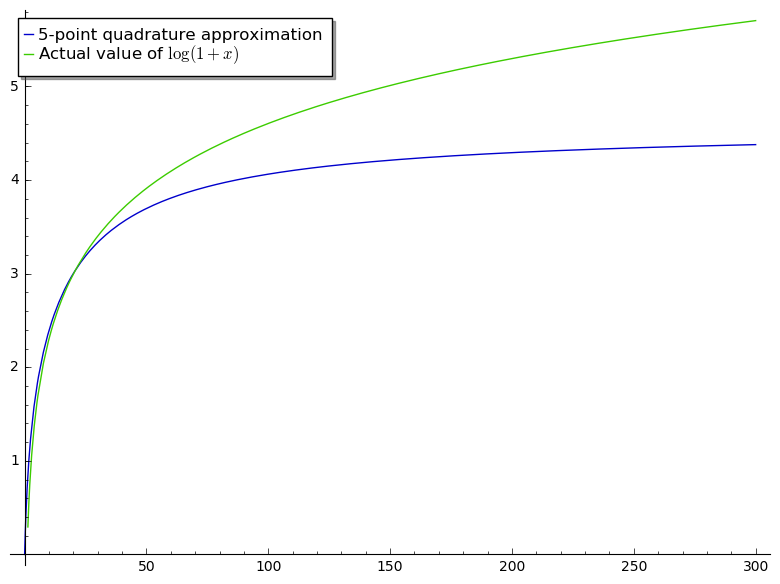
\includegraphics[width=.8\linewidth]{figures/StandardQuadrature.png}
%     \caption{Graph of $\log{(1+x)}$ and the approximation in equation \ref{eq:standardquadrature}}
%     \label{fig:standardquadrature}
% \end{figure}
\begin{figure}[!ht]
    \centering
	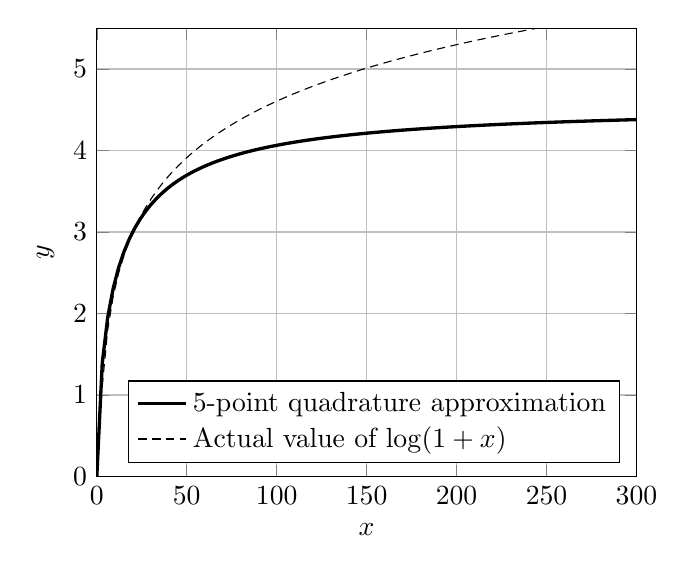
\begin{tikzpicture}
		\begin{axis}[
			% height=6cm, width=9cm,
			xmin=0, xmax=300,
			ymin=0, ymax=5.5, ytick={0,...,6},
			xlabel={$x$}, ylabel={$y$},
			grid=major,
			legend pos=south east,
			legend cell align=left,
		]
		\addplot[very thick, domain=0:300, samples=100]{1/30*(137*x^5 + 2310*x^4 + 9870*x^3 + 15120*x^2 + 7560*x)/(x^5 + 30*x^4 + 210*x^3 + 560*x^2 + 630*x + 252)};
		\addplot[densely dashed, domain=0:300, samples=100]{ln(x)};
		\legend{5-point quadrature approximation, Actual value of $\log(1+x)$}
		\end{axis}
	\end{tikzpicture}%
    \caption{Graph of $\log{(1+x)}$ and the approximation in Equation~\ref{eq:standardquadrature}}
    \label{fig:standardquadrature}
\end{figure}

As we only need accuracy for arguments $x \in [0, 255]$, we can scale the approximation by a constant factor $\alpha$ as follows:
\begin{align*}
  \log{(1+x)} &= \log{\left(\frac{\alpha + \alpha x}{\alpha}\right)}\\
  &= \log{(\alpha + \alpha x)} - \log{\alpha}\\
  &= \log{\left(\alpha+\frac{\alpha}{n}\right)} - \log{\alpha}\\
  &= \log{\left(\frac{\alpha n + \alpha}{n}\right)} - \log{\alpha}\\
  &= \int_{n}^{\alpha n + \alpha}{\frac{1}{x}\diff x} - \log{\alpha}
\end{align*}

Applying the five-point Gauss--Legendre quadrature rule with $\alpha = 1/20$ using SageMath 8.3, we arrive at the approximation:
\begin{align}\label{eq:scaledquadrature}
  \begin{split}
    &\log(1+x) \\
    &\approx \frac{137x^5 + 33185x^4 + 931370x^3 - 13403630x^2 - 289469315x - 713567363}
    {30(x^5 + 505x^4 + 42010x^3 + 923010x^2 + 5722005x + 8040501)} \\
    &+ \log{20}
  \end{split}
\end{align}

Figure~\ref{fig:scaledquadrature} is a graph of the absolute error of the scaled approximation and the exact value of $\log{(1+x)}$. Using SageMath 8.3, it was numerically determined that the maximum absolute error of this approximation in the range $x\in[0,255]$ is approximately $0.0103315865985758$, occurring at $x=255$. This is an improvement from the approximation in Equation~\ref{eq:standardquadrature}, which has a maximum absolute error of $1.19717868468392$, similarly occurring at $x=255$.

% \begin{figure}[h]
%     \centering
%     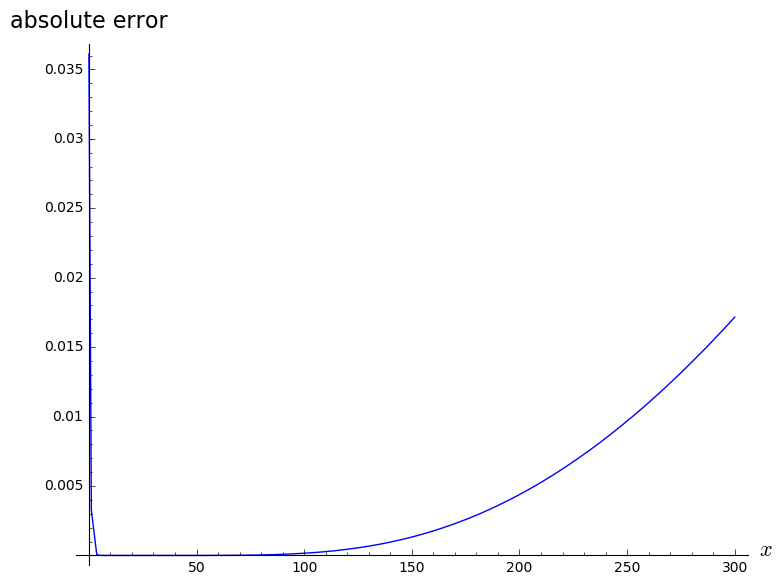
\includegraphics[width=.9\linewidth]{figures/ModifiedQuadratureAbsoluteError.png}
%     \caption{Graph of the absolute error of $\log{(1+x)}$ and the approximation in equation \ref{eq:scaledquadrature}}
%     \label{fig:scaledquadrature}
% \end{figure}
\begin{figure}[h]
    \centering
    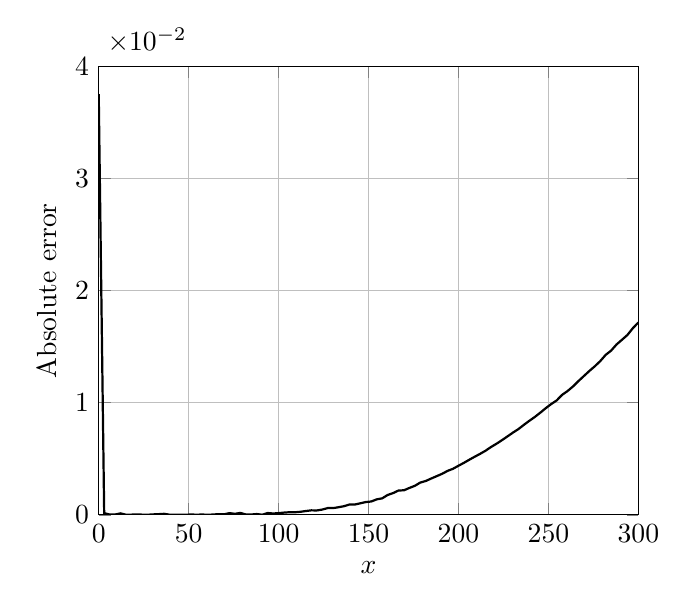
\begin{tikzpicture}
		\begin{axis}[
			% height=6cm, width=9cm,
			xmin=0, xmax=300,
			ymin=0, ymax=0.04,
			xlabel={$x$}, ylabel={Absolute error},
			grid=major,
			legend pos=south east,
			legend cell align=left,
			tick scale binop=\times,
		]
		\addplot[thick, domain=0:300, samples=100]{abs((1/30*(137*x^5 + 33185*x^4 + 931370*x^3 - 13403630*x^2 - 289469315*x - 713567363)/(x^5 + 505*x^4 + 42010*x^3 + 923010*x^2 + 5722005*x + 8040501))-ln((1/20)+(1/20)*x))};
		\end{axis}
	\end{tikzpicture}%
    \caption{Graph of the absolute error of $\log{(1+x)}$ and the approximation in Equation~\ref{eq:scaledquadrature}}
    \label{fig:scaledquadrature}
\end{figure}

\section{Approximation for $x^\gamma$}
\label{sec:approx-pwr}
To approximate $x^\gamma$ for any $\gamma \in \mathbb{R}$, we rewrite $x^\gamma$ as follows:
\begin{align*}
  x^\gamma = e^{\log{x^\gamma}} = e^{\gamma\log{x}}.
\end{align*}

This expression can then be approximated using the Maclaurin series expansion for $e^x$, which converges for all $x$.
\begin{align*}
  e^x &= \sum_{n=0}^{\infty}{\frac{x^n}{n!}}\\
  \Rightarrow \quad e^{\gamma\log{x}} &= \sum_{n=0}^{\infty}{\frac{(\gamma\log{x})^n}{n!}}
\end{align*}

As we already have an approximation for the natural logarithm, we can evaluate partial sums of the above infinite series to arrive at approximations for $x^\gamma$.